\documentclass{standalone}
\usepackage{tikz}
\usetikzlibrary{patterns}
\usetikzlibrary{positioning}
\usetikzlibrary{patterns, positioning}
\usetikzlibrary{shapes.misc}
\usepackage[outline]{contour}
\contourlength{1.5pt} 
\usetikzlibrary{calc}
        \usepackage{relsize}
        \tikzset{fontscale/.style = {font=\relsize{#1}}}

\begin{document}
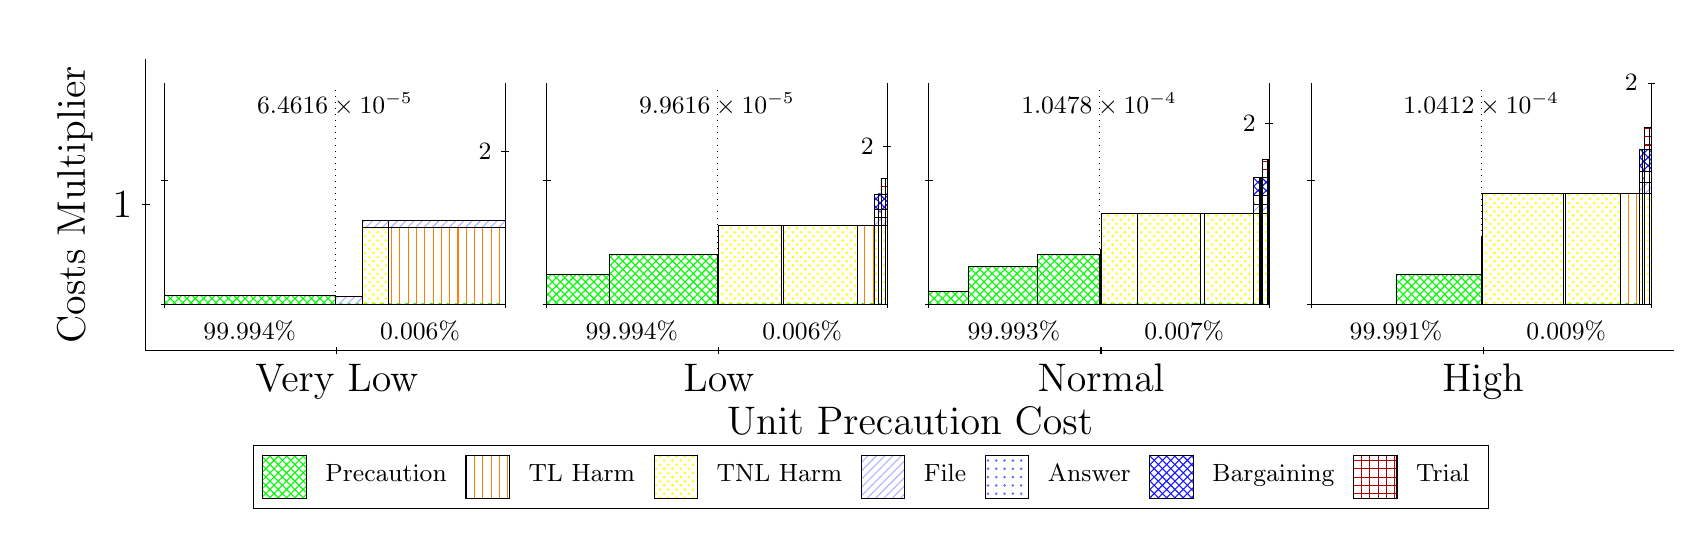
\begin{tikzpicture}
\clip(-0.5,-1.1) rectangle +(20.91,6.2);
\draw[black] (1,1) -- (1,4.7);
\node[rotate=90, fontscale=2, anchor=center] at (0.1, 2.85) {Costs Multiplier};
\draw[black] (0.95,2.85) -- (1.05,2.85);
\node[fontscale=2, anchor=east] at (0.95, 2.85) {1};

\draw[black] (1,1) -- (20.41,1);
\node[fontscale=2, anchor=center] at (10.705, 0.1) {Unit Precaution Cost};
\draw[black] (3.4263,0.95) -- (3.4263,1.05);
\node[fontscale=2, anchor=north] at (3.4263, 0.95) {Very Low};
\draw[black] (8.2788,0.95) -- (8.2788,1.05);
\node[fontscale=2, anchor=north] at (8.2788, 0.95) {Low};
\draw[black] (13.131,0.95) -- (13.131,1.05);
\node[fontscale=2, anchor=north] at (13.131, 0.95) {Normal};
\draw[black] (17.984,0.95) -- (17.984,1.05);
\node[fontscale=2, anchor=north] at (17.984, 0.95) {High};


\draw[pattern=crosshatch, pattern color=green,draw=black,very thin] (1.2381,1.592) rectangle (3.4013,1.7022);
\draw[pattern=crosshatch, pattern color=green,draw=black,very thin] (3.4013,1.592) rectangle (3.7531,1.592);
\draw[pattern=north east lines, pattern color=blue!30,draw=black,very thin] (3.4013,1.592) rectangle (3.7531,1.6888);
\draw[pattern=crosshatch, pattern color=green,draw=black,very thin] (3.7531,1.592) rectangle (4.0772,1.592);
\draw[pattern=crosshatch dots, pattern color=yellow,draw=black,very thin] (3.7531,1.592) rectangle (4.0772,2.5599);
\draw[pattern=north east lines, pattern color=blue!30,draw=black,very thin] (3.7531,2.5599) rectangle (4.0772,2.6567);
\draw[pattern=crosshatch, pattern color=green,draw=black,very thin] (4.0772,1.592) rectangle (5.5644,1.592);
\draw[pattern=vertical lines, pattern color=orange,draw=black,very thin] (4.0772,1.592) rectangle (5.5644,2.5599);
\draw[pattern=north east lines, pattern color=blue!30,draw=black,very thin] (4.0772,2.5599) rectangle (5.5644,2.6567);
\node[font=\small,text=black,anchor=north] at (3.4013, 4.4) {$6.4616\times 10^{-5}$};
\draw[black,very thin] (1.2381,1.592) -- (1.2381,4.4);
\draw[black,very thin] (1.1881,1.592) -- (1.2881,1.592);
\node[font=\small,text=black, anchor=west] at (1.1881, 1.592) {};
\draw[black,very thin] (1.1881,3.1665) -- (1.2881,3.1665);
\node[font=\small,text=black, anchor=west] at (1.1881, 3.1665) {};

\draw[black,dotted,very thin] (3.4013,1.6762) -- (3.4013,4.3158);
\draw[black,very thin] (5.5644,1.592) -- (5.5644,4.4);
\draw[black,very thin] (5.5144,3.5277) -- (5.6144,3.5277);
\node[font=\small,text=black, anchor=east] at (5.5144, 3.5277) {\contour{white}{2}};

\draw[black,very thin] (1.2381,1.592) -- (5.5644,1.592);
\draw[black,very thin] (1.2381,1.542) -- (1.2381,1.642);
\node[font=\small,text=black, anchor=north] at (1.2381, 1.542) {};
\draw[black,very thin] (5.5644,1.542) -- (5.5644,1.642);
\node[font=\small,text=black, anchor=north] at (5.5644, 1.542) {};

\node[font=\small,text=black,anchor=south] at (2.3197, 0.992) {99.994\%};
\node[font=\small,text=black,anchor=south] at (4.4828, 0.992) {0.006\%};

\draw[pattern=crosshatch, pattern color=green,draw=black,very thin] (6.0906,1.592) rectangle (6.8804,1.9699);
\draw[pattern=crosshatch, pattern color=green,draw=black,very thin] (6.8804,1.592) rectangle (8.2538,2.2218);
\draw[pattern=crosshatch, pattern color=green,draw=black,very thin] (8.2538,1.592) rectangle (8.2647,1.592);
\draw[pattern=north east lines, pattern color=blue!30,draw=black,very thin] (8.2538,1.592) rectangle (8.2647,1.6919);
\draw[pattern=dots,  pattern color=blue!60,draw=black,very thin] (8.2538,1.6919) rectangle (8.2647,1.7918);
\draw[pattern=crosshatch,      pattern color=blue!90,draw=black,very thin] (8.2538,1.7918) rectangle (8.2647,1.9915);
\draw[pattern=crosshatch, pattern color=green,draw=black,very thin] (8.2647,1.592) rectangle (8.2754,1.592);
\draw[pattern=north east lines, pattern color=blue!30,draw=black,very thin] (8.2647,1.592) rectangle (8.2754,1.6919);
\draw[pattern=dots,  pattern color=blue!60,draw=black,very thin] (8.2647,1.6919) rectangle (8.2754,1.7918);
\draw[pattern=crosshatch,      pattern color=blue!90,draw=black,very thin] (8.2647,1.7918) rectangle (8.2754,1.9915);
\draw[pattern=grid,            pattern color=red!70!black,draw=black,very thin] (8.2647,1.9915) rectangle (8.2754,2.1913);
\draw[pattern=crosshatch, pattern color=green,draw=black,very thin] (8.2754,1.592) rectangle (9.0764,1.592);
\draw[pattern=crosshatch dots, pattern color=yellow,draw=black,very thin] (8.2754,1.592) rectangle (9.0764,2.5908);
\draw[pattern=crosshatch, pattern color=green,draw=black,very thin] (9.0764,1.592) rectangle (9.0985,1.592);
\draw[pattern=vertical lines, pattern color=orange,draw=black,very thin] (9.0764,1.592) rectangle (9.0985,2.5908);
\draw[pattern=crosshatch, pattern color=green,draw=black,very thin] (9.0985,1.592) rectangle (10.038,1.592);
\draw[pattern=crosshatch dots, pattern color=yellow,draw=black,very thin] (9.0985,1.592) rectangle (10.038,2.5908);
\draw[pattern=crosshatch, pattern color=green,draw=black,very thin] (10.038,1.592) rectangle (10.257,1.592);
\draw[pattern=vertical lines, pattern color=orange,draw=black,very thin] (10.038,1.592) rectangle (10.257,2.5908);
\draw[pattern=crosshatch, pattern color=green,draw=black,very thin] (10.257,1.592) rectangle (10.303,1.592);
\draw[pattern=crosshatch dots, pattern color=yellow,draw=black,very thin] (10.257,1.592) rectangle (10.303,2.5908);
\draw[pattern=north east lines, pattern color=blue!30,draw=black,very thin] (10.257,2.5908) rectangle (10.303,2.6907);
\draw[pattern=dots,  pattern color=blue!60,draw=black,very thin] (10.257,2.6907) rectangle (10.303,2.7906);
\draw[pattern=crosshatch,      pattern color=blue!90,draw=black,very thin] (10.257,2.7906) rectangle (10.303,2.9903);
\draw[pattern=crosshatch, pattern color=green,draw=black,very thin] (10.303,1.592) rectangle (10.337,1.592);
\draw[pattern=vertical lines, pattern color=orange,draw=black,very thin] (10.303,1.592) rectangle (10.337,2.5908);
\draw[pattern=north east lines, pattern color=blue!30,draw=black,very thin] (10.303,2.5908) rectangle (10.337,2.6907);
\draw[pattern=dots,  pattern color=blue!60,draw=black,very thin] (10.303,2.6907) rectangle (10.337,2.7906);
\draw[pattern=crosshatch,      pattern color=blue!90,draw=black,very thin] (10.303,2.7906) rectangle (10.337,2.9903);
\draw[pattern=crosshatch, pattern color=green,draw=black,very thin] (10.337,1.592) rectangle (10.397,1.592);
\draw[pattern=crosshatch dots, pattern color=yellow,draw=black,very thin] (10.337,1.592) rectangle (10.397,2.5908);
\draw[pattern=north east lines, pattern color=blue!30,draw=black,very thin] (10.337,2.5908) rectangle (10.397,2.6907);
\draw[pattern=dots,  pattern color=blue!60,draw=black,very thin] (10.337,2.6907) rectangle (10.397,2.7906);
\draw[pattern=crosshatch,      pattern color=blue!90,draw=black,very thin] (10.337,2.7906) rectangle (10.397,2.9903);
\draw[pattern=grid,            pattern color=red!70!black,draw=black,very thin] (10.337,2.9903) rectangle (10.397,3.1901);
\draw[pattern=crosshatch, pattern color=green,draw=black,very thin] (10.397,1.592) rectangle (10.417,1.592);
\draw[pattern=vertical lines, pattern color=orange,draw=black,very thin] (10.397,1.592) rectangle (10.417,2.5908);
\draw[pattern=north east lines, pattern color=blue!30,draw=black,very thin] (10.397,2.5908) rectangle (10.417,2.6907);
\draw[pattern=dots,  pattern color=blue!60,draw=black,very thin] (10.397,2.6907) rectangle (10.417,2.7906);
\draw[pattern=crosshatch,      pattern color=blue!90,draw=black,very thin] (10.397,2.7906) rectangle (10.417,2.9903);
\draw[pattern=grid,            pattern color=red!70!black,draw=black,very thin] (10.397,2.9903) rectangle (10.417,3.1901);
\node[font=\small,text=black,anchor=north] at (8.2538, 4.4) {$9.9616\times 10^{-5}$};
\draw[black,very thin] (6.0906,1.592) -- (6.0906,4.4);
\draw[black,very thin] (6.0406,1.592) -- (6.1406,1.592);
\node[font=\small,text=black, anchor=west] at (6.0406, 1.592) {};
\draw[black,very thin] (6.0406,3.1665) -- (6.1406,3.1665);
\node[font=\small,text=black, anchor=west] at (6.0406, 3.1665) {};

\draw[black,dotted,very thin] (8.2538,1.6762) -- (8.2538,4.3158);
\draw[black,very thin] (10.417,1.592) -- (10.417,4.4);
\draw[black,very thin] (10.367,3.5896) -- (10.467,3.5896);
\node[font=\small,text=black, anchor=east] at (10.367, 3.5896) {\contour{white}{2}};

\draw[black,very thin] (6.0906,1.592) -- (10.417,1.592);
\draw[black,very thin] (6.0906,1.542) -- (6.0906,1.642);
\node[font=\small,text=black, anchor=north] at (6.0906, 1.542) {};
\draw[black,very thin] (10.417,1.542) -- (10.417,1.642);
\node[font=\small,text=black, anchor=north] at (10.417, 1.542) {};

\node[font=\small,text=black,anchor=south] at (7.1722, 0.992) {99.994\%};
\node[font=\small,text=black,anchor=south] at (9.3353, 0.992) {0.006\%};

\draw[pattern=crosshatch, pattern color=green,draw=black,very thin] (10.943,1.592) rectangle (11.441,1.7494);
\draw[pattern=crosshatch, pattern color=green,draw=black,very thin] (11.441,1.592) rectangle (12.316,2.0643);
\draw[pattern=crosshatch, pattern color=green,draw=black,very thin] (12.316,1.592) rectangle (13.106,2.2218);
\draw[pattern=crosshatch, pattern color=green,draw=black,very thin] (13.106,1.592) rectangle (13.117,1.592);
\draw[pattern=north east lines, pattern color=blue!30,draw=black,very thin] (13.106,1.592) rectangle (13.117,1.7066);
\draw[pattern=dots,  pattern color=blue!60,draw=black,very thin] (13.106,1.7066) rectangle (13.117,1.8212);
\draw[pattern=crosshatch,      pattern color=blue!90,draw=black,very thin] (13.106,1.8212) rectangle (13.117,2.0504);
\draw[pattern=crosshatch, pattern color=green,draw=black,very thin] (13.117,1.592) rectangle (13.121,1.592);
\draw[pattern=north east lines, pattern color=blue!30,draw=black,very thin] (13.117,1.592) rectangle (13.121,1.7066);
\draw[pattern=dots,  pattern color=blue!60,draw=black,very thin] (13.117,1.7066) rectangle (13.121,1.8212);
\draw[pattern=crosshatch,      pattern color=blue!90,draw=black,very thin] (13.117,1.8212) rectangle (13.121,2.0504);
\draw[pattern=crosshatch, pattern color=green,draw=black,very thin] (13.121,1.592) rectangle (13.128,1.592);
\draw[pattern=north east lines, pattern color=blue!30,draw=black,very thin] (13.121,1.592) rectangle (13.128,1.7066);
\draw[pattern=dots,  pattern color=blue!60,draw=black,very thin] (13.121,1.7066) rectangle (13.128,1.8212);
\draw[pattern=crosshatch,      pattern color=blue!90,draw=black,very thin] (13.121,1.8212) rectangle (13.128,2.0504);
\draw[pattern=grid,            pattern color=red!70!black,draw=black,very thin] (13.121,2.0504) rectangle (13.128,2.2796);
\draw[pattern=crosshatch, pattern color=green,draw=black,very thin] (13.128,1.592) rectangle (13.131,1.592);
\draw[pattern=north east lines, pattern color=blue!30,draw=black,very thin] (13.128,1.592) rectangle (13.131,1.7066);
\draw[pattern=dots,  pattern color=blue!60,draw=black,very thin] (13.128,1.7066) rectangle (13.131,1.8212);
\draw[pattern=crosshatch,      pattern color=blue!90,draw=black,very thin] (13.128,1.8212) rectangle (13.131,2.0504);
\draw[pattern=grid,            pattern color=red!70!black,draw=black,very thin] (13.128,2.0504) rectangle (13.131,2.2797);
\draw[pattern=crosshatch, pattern color=green,draw=black,very thin] (13.131,1.592) rectangle (13.595,1.592);
\draw[pattern=crosshatch dots, pattern color=yellow,draw=black,very thin] (13.131,1.592) rectangle (13.595,2.738);
\draw[pattern=crosshatch, pattern color=green,draw=black,very thin] (13.595,1.592) rectangle (13.598,1.592);
\draw[pattern=vertical lines, pattern color=orange,draw=black,very thin] (13.595,1.592) rectangle (13.598,2.738);
\draw[pattern=crosshatch, pattern color=green,draw=black,very thin] (13.598,1.592) rectangle (14.387,1.592);
\draw[pattern=crosshatch dots, pattern color=yellow,draw=black,very thin] (13.598,1.592) rectangle (14.387,2.7381);
\draw[pattern=crosshatch, pattern color=green,draw=black,very thin] (14.387,1.592) rectangle (14.444,1.592);
\draw[pattern=vertical lines, pattern color=orange,draw=black,very thin] (14.387,1.592) rectangle (14.444,2.7381);
\draw[pattern=crosshatch, pattern color=green,draw=black,very thin] (14.444,1.592) rectangle (15.062,1.592);
\draw[pattern=crosshatch dots, pattern color=yellow,draw=black,very thin] (14.444,1.592) rectangle (15.062,2.7381);
\draw[pattern=crosshatch, pattern color=green,draw=black,very thin] (15.062,1.592) rectangle (15.146,1.592);
\draw[pattern=crosshatch dots, pattern color=yellow,draw=black,very thin] (15.062,1.592) rectangle (15.146,2.738);
\draw[pattern=north east lines, pattern color=blue!30,draw=black,very thin] (15.062,2.738) rectangle (15.146,2.8527);
\draw[pattern=dots,  pattern color=blue!60,draw=black,very thin] (15.062,2.8527) rectangle (15.146,2.9673);
\draw[pattern=crosshatch,      pattern color=blue!90,draw=black,very thin] (15.062,2.9673) rectangle (15.146,3.1965);
\draw[pattern=crosshatch, pattern color=green,draw=black,very thin] (15.146,1.592) rectangle (15.158,1.592);
\draw[pattern=vertical lines, pattern color=orange,draw=black,very thin] (15.146,1.592) rectangle (15.158,2.738);
\draw[pattern=north east lines, pattern color=blue!30,draw=black,very thin] (15.146,2.738) rectangle (15.158,2.8527);
\draw[pattern=dots,  pattern color=blue!60,draw=black,very thin] (15.146,2.8527) rectangle (15.158,2.9673);
\draw[pattern=crosshatch,      pattern color=blue!90,draw=black,very thin] (15.146,2.9673) rectangle (15.158,3.1965);
\draw[pattern=crosshatch, pattern color=green,draw=black,very thin] (15.158,1.592) rectangle (15.166,1.592);
\draw[pattern=crosshatch dots, pattern color=yellow,draw=black,very thin] (15.158,1.592) rectangle (15.166,2.7381);
\draw[pattern=north east lines, pattern color=blue!30,draw=black,very thin] (15.158,2.7381) rectangle (15.166,2.8527);
\draw[pattern=dots,  pattern color=blue!60,draw=black,very thin] (15.158,2.8527) rectangle (15.166,2.9673);
\draw[pattern=crosshatch,      pattern color=blue!90,draw=black,very thin] (15.158,2.9673) rectangle (15.166,3.1965);
\draw[pattern=crosshatch, pattern color=green,draw=black,very thin] (15.166,1.592) rectangle (15.183,1.592);
\draw[pattern=vertical lines, pattern color=orange,draw=black,very thin] (15.166,1.592) rectangle (15.183,2.7381);
\draw[pattern=north east lines, pattern color=blue!30,draw=black,very thin] (15.166,2.7381) rectangle (15.183,2.8527);
\draw[pattern=dots,  pattern color=blue!60,draw=black,very thin] (15.166,2.8527) rectangle (15.183,2.9673);
\draw[pattern=crosshatch,      pattern color=blue!90,draw=black,very thin] (15.166,2.9673) rectangle (15.183,3.1965);
\draw[pattern=crosshatch, pattern color=green,draw=black,very thin] (15.183,1.592) rectangle (15.244,1.592);
\draw[pattern=crosshatch dots, pattern color=yellow,draw=black,very thin] (15.183,1.592) rectangle (15.244,2.738);
\draw[pattern=north east lines, pattern color=blue!30,draw=black,very thin] (15.183,2.738) rectangle (15.244,2.8527);
\draw[pattern=dots,  pattern color=blue!60,draw=black,very thin] (15.183,2.8527) rectangle (15.244,2.9673);
\draw[pattern=crosshatch,      pattern color=blue!90,draw=black,very thin] (15.183,2.9673) rectangle (15.244,3.1965);
\draw[pattern=grid,            pattern color=red!70!black,draw=black,very thin] (15.183,3.1965) rectangle (15.244,3.4257);
\draw[pattern=crosshatch, pattern color=green,draw=black,very thin] (15.244,1.592) rectangle (15.252,1.592);
\draw[pattern=vertical lines, pattern color=orange,draw=black,very thin] (15.244,1.592) rectangle (15.252,2.738);
\draw[pattern=north east lines, pattern color=blue!30,draw=black,very thin] (15.244,2.738) rectangle (15.252,2.8527);
\draw[pattern=dots,  pattern color=blue!60,draw=black,very thin] (15.244,2.8527) rectangle (15.252,2.9673);
\draw[pattern=crosshatch,      pattern color=blue!90,draw=black,very thin] (15.244,2.9673) rectangle (15.252,3.1965);
\draw[pattern=grid,            pattern color=red!70!black,draw=black,very thin] (15.244,3.1965) rectangle (15.252,3.4257);
\draw[pattern=crosshatch, pattern color=green,draw=black,very thin] (15.252,1.592) rectangle (15.262,1.592);
\draw[pattern=crosshatch dots, pattern color=yellow,draw=black,very thin] (15.252,1.592) rectangle (15.262,2.7381);
\draw[pattern=north east lines, pattern color=blue!30,draw=black,very thin] (15.252,2.7381) rectangle (15.262,2.8527);
\draw[pattern=dots,  pattern color=blue!60,draw=black,very thin] (15.252,2.8527) rectangle (15.262,2.9673);
\draw[pattern=crosshatch,      pattern color=blue!90,draw=black,very thin] (15.252,2.9673) rectangle (15.262,3.1965);
\draw[pattern=grid,            pattern color=red!70!black,draw=black,very thin] (15.252,3.1965) rectangle (15.262,3.4257);
\draw[pattern=crosshatch, pattern color=green,draw=black,very thin] (15.262,1.592) rectangle (15.269,1.592);
\draw[pattern=vertical lines, pattern color=orange,draw=black,very thin] (15.262,1.592) rectangle (15.269,2.7381);
\draw[pattern=north east lines, pattern color=blue!30,draw=black,very thin] (15.262,2.7381) rectangle (15.269,2.8527);
\draw[pattern=dots,  pattern color=blue!60,draw=black,very thin] (15.262,2.8527) rectangle (15.269,2.9673);
\draw[pattern=crosshatch,      pattern color=blue!90,draw=black,very thin] (15.262,2.9673) rectangle (15.269,3.1965);
\draw[pattern=grid,            pattern color=red!70!black,draw=black,very thin] (15.262,3.1965) rectangle (15.269,3.4257);
\node[font=\small,text=black,anchor=north] at (13.106, 4.4) {$1.0478\times 10^{-4}$};
\draw[black,very thin] (10.943,1.592) -- (10.943,4.4);
\draw[black,very thin] (10.893,1.592) -- (10.993,1.592);
\node[font=\small,text=black, anchor=west] at (10.893, 1.592) {};
\draw[black,very thin] (10.893,3.1665) -- (10.993,3.1665);
\node[font=\small,text=black, anchor=west] at (10.893, 3.1665) {};

\draw[black,dotted,very thin] (13.106,1.6762) -- (13.106,4.3158);
\draw[black,very thin] (15.269,1.592) -- (15.269,4.4);
\draw[black,very thin] (15.219,3.8841) -- (15.319,3.8841);
\node[font=\small,text=black, anchor=east] at (15.219, 3.8841) {\contour{white}{2}};

\draw[black,very thin] (10.943,1.592) -- (15.269,1.592);
\draw[black,very thin] (10.943,1.542) -- (10.943,1.642);
\node[font=\small,text=black, anchor=north] at (10.943, 1.542) {};
\draw[black,very thin] (15.269,1.542) -- (15.269,1.642);
\node[font=\small,text=black, anchor=north] at (15.269, 1.542) {};

\node[font=\small,text=black,anchor=south] at (12.025, 0.992) {99.993\%};
\node[font=\small,text=black,anchor=south] at (14.188, 0.992) {0.007\%};

\draw[pattern=crosshatch, pattern color=green,draw=black,very thin] (16.877,1.592) rectangle (17.959,1.9699);
\draw[pattern=north east lines, pattern color=blue!30,draw=black,very thin] (17.959,1.592) rectangle (17.965,1.7324);
\draw[pattern=dots,  pattern color=blue!60,draw=black,very thin] (17.959,1.7324) rectangle (17.965,1.8728);
\draw[pattern=crosshatch,      pattern color=blue!90,draw=black,very thin] (17.959,1.8728) rectangle (17.965,2.1536);
\draw[pattern=north east lines, pattern color=blue!30,draw=black,very thin] (17.965,1.592) rectangle (17.974,1.7324);
\draw[pattern=dots,  pattern color=blue!60,draw=black,very thin] (17.965,1.7324) rectangle (17.974,1.8728);
\draw[pattern=crosshatch,      pattern color=blue!90,draw=black,very thin] (17.965,1.8728) rectangle (17.974,2.1536);
\draw[pattern=grid,            pattern color=red!70!black,draw=black,very thin] (17.965,2.1536) rectangle (17.974,2.4344);
\draw[pattern=crosshatch dots, pattern color=yellow,draw=black,very thin] (17.974,1.592) rectangle (19.008,2.996);
\draw[pattern=vertical lines, pattern color=orange,draw=black,very thin] (19.008,1.592) rectangle (19.033,2.996);
\draw[pattern=crosshatch, pattern color=green,draw=black,very thin] (19.033,1.592) rectangle (19.723,1.592);
\draw[pattern=crosshatch dots, pattern color=yellow,draw=black,very thin] (19.033,1.592) rectangle (19.723,2.996);
\draw[pattern=crosshatch, pattern color=green,draw=black,very thin] (19.723,1.592) rectangle (19.968,1.592);
\draw[pattern=vertical lines, pattern color=orange,draw=black,very thin] (19.723,1.592) rectangle (19.968,2.996);
\draw[pattern=crosshatch dots, pattern color=yellow,draw=black,very thin] (19.968,1.592) rectangle (20.004,2.996);
\draw[pattern=north east lines, pattern color=blue!30,draw=black,very thin] (19.968,2.996) rectangle (20.004,3.1364);
\draw[pattern=dots,  pattern color=blue!60,draw=black,very thin] (19.968,3.1364) rectangle (20.004,3.2768);
\draw[pattern=crosshatch,      pattern color=blue!90,draw=black,very thin] (19.968,3.2768) rectangle (20.004,3.5576);
\draw[pattern=vertical lines, pattern color=orange,draw=black,very thin] (20.004,1.592) rectangle (20.035,2.996);
\draw[pattern=north east lines, pattern color=blue!30,draw=black,very thin] (20.004,2.996) rectangle (20.035,3.1364);
\draw[pattern=dots,  pattern color=blue!60,draw=black,very thin] (20.004,3.1364) rectangle (20.035,3.2768);
\draw[pattern=crosshatch,      pattern color=blue!90,draw=black,very thin] (20.004,3.2768) rectangle (20.035,3.5576);
\draw[pattern=crosshatch dots, pattern color=yellow,draw=black,very thin] (20.035,1.592) rectangle (20.094,2.996);
\draw[pattern=north east lines, pattern color=blue!30,draw=black,very thin] (20.035,2.996) rectangle (20.094,3.1364);
\draw[pattern=dots,  pattern color=blue!60,draw=black,very thin] (20.035,3.1364) rectangle (20.094,3.2768);
\draw[pattern=crosshatch,      pattern color=blue!90,draw=black,very thin] (20.035,3.2768) rectangle (20.094,3.5576);
\draw[pattern=grid,            pattern color=red!70!black,draw=black,very thin] (20.035,3.5576) rectangle (20.094,3.8384);
\draw[pattern=vertical lines, pattern color=orange,draw=black,very thin] (20.094,1.592) rectangle (20.122,2.996);
\draw[pattern=north east lines, pattern color=blue!30,draw=black,very thin] (20.094,2.996) rectangle (20.122,3.1364);
\draw[pattern=dots,  pattern color=blue!60,draw=black,very thin] (20.094,3.1364) rectangle (20.122,3.2768);
\draw[pattern=crosshatch,      pattern color=blue!90,draw=black,very thin] (20.094,3.2768) rectangle (20.122,3.5576);
\draw[pattern=grid,            pattern color=red!70!black,draw=black,very thin] (20.094,3.5576) rectangle (20.122,3.8384);
\node[font=\small,text=black,anchor=north] at (17.959, 4.4) {$1.0412\times 10^{-4}$};
\draw[black,very thin] (15.796,1.592) -- (15.796,4.4);
\draw[black,very thin] (15.746,1.592) -- (15.846,1.592);
\node[font=\small,text=black, anchor=west] at (15.746, 1.592) {};
\draw[black,very thin] (15.746,3.1664) -- (15.846,3.1664);
\node[font=\small,text=black, anchor=west] at (15.746, 3.1664) {};

\draw[black,dotted,very thin] (17.959,1.6762) -- (17.959,4.3158);
\draw[black,very thin] (20.122,1.592) -- (20.122,4.4);
\draw[black,very thin] (20.072,4.4) -- (20.172,4.4);
\node[font=\small,text=black, anchor=east] at (20.072, 4.4) {\contour{white}{2}};

\draw[black,very thin] (15.796,1.592) -- (20.122,1.592);
\draw[black,very thin] (15.796,1.542) -- (15.796,1.642);
\node[font=\small,text=black, anchor=north] at (15.796, 1.542) {};
\draw[black,very thin] (20.122,1.542) -- (20.122,1.642);
\node[font=\small,text=black, anchor=north] at (20.122, 1.542) {};

\node[font=\small,text=black,anchor=south] at (16.877, 0.992) {99.991\%};
\node[font=\small,text=black,anchor=south] at (19.04, 0.992) {0.009\%};

\coordinate (LegendAnchor) at (10.205000000000002,0);
\begin{scope}[align=center]
\matrix[scale=0.6,draw=black,below=0.2cm of LegendAnchor,nodes={draw},column sep=0.12cm]{
\node[rectangle,draw,minimum width=0.55cm,minimum height=0.55cm,pattern=crosshatch, pattern color=green]{}; &
        \node[draw=none,font=\small]{Precaution}; &
\node[rectangle,draw,minimum width=0.55cm,minimum height=0.55cm,pattern=vertical lines, pattern color=orange]{}; &
        \node[draw=none,font=\small]{TL Harm}; &
\node[rectangle,draw,minimum width=0.55cm,minimum height=0.55cm,pattern=crosshatch dots, pattern color=yellow]{}; &
        \node[draw=none,font=\small]{TNL Harm}; &
\node[rectangle,draw,minimum width=0.55cm,minimum height=0.55cm,pattern=north east lines, pattern color=blue!30]{}; &
        \node[draw=none,font=\small]{File}; &
\node[rectangle,draw,minimum width=0.55cm,minimum height=0.55cm,pattern=dots, pattern color=blue!60]{}; &
        \node[draw=none,font=\small]{Answer}; &
\node[rectangle,draw,minimum width=0.55cm,minimum height=0.55cm,pattern=crosshatch, pattern color=blue!90]{}; &
        \node[draw=none,font=\small]{Bargaining}; &
\node[rectangle,draw,minimum width=0.55cm,minimum height=0.55cm,pattern=grid, pattern color=red!70!black]{}; &
        \node[draw=none,font=\small]{Trial}; \\
};\end{scope}

\end{tikzpicture}
\end{document}